\documentclass[12pt,a4paper]{article}

% --- LuaLaTeX（日本語対応）。原ノ味フォントはTeX Liveに入っているので、Mac・Windows・Overleafで同じ見た目になる ---
\usepackage{luatexja}
\usepackage[haranoaji]{luatexja-preset}

\usepackage{amsmath,amssymb,amsfonts}
\usepackage{graphicx}
\usepackage{booktabs}
\usepackage{hyperref}
\usepackage{natbib}
\usepackage[margin=1in]{geometry}
\usepackage{setspace}
\usepackage{caption}
\usepackage{float}
\usepackage{textcomp} % \textyen

\hypersetup{unicode=true}

\onehalfspacing
\renewcommand{\abstractname}{要旨}

\title{通貨政治・貿易摩擦と日米自動車産業における為替エクスポージャー：LP-IVとイベントスタディによる証拠（日本語訳）}
\author{久保田 荘\\東北大学}
\date{2026年9月23日}

\begin{document}

\maketitle

\begin{abstract}
日米自動車関係は、為替レート、通商政策、企業戦略が相互に進化してきた典型例である。1980年代には、円安は日本の輸出企業にとって構造的な優位と広く見なされ、米国の政策当局は二国間の自動車貿易赤字を不公正競争の証左として位置付けた。しかし、その後40年にわたる適応---自主規制（Voluntary Export Restraints: VERs）、プラザ合意、繰り返される関税脅威、北米における「トランスプラント（現地生産）」の拡大---は、日本の自動車メーカーがどこで生産し、調達し、収益を得るのかを根本的に変えてきた。

本稿は、この歴史的変容が現代の金融市場における感応度にどのように写像されているかを定量化する。主要5社（トヨタ、ホンダ、日産、ゼネラル・モーターズ、フォード）とUSD/JPY為替レートについて、過去10年の日次データを用い、Local Projections Instrumental Variables（LP-IV）により、為替ショックが株式価値に及ぼす動学的な因果効果を推定する。為替変動と株式収益率の内生性に対処するため、USD/JPYの変化を米国2年国債利回りのイノベーション---金融政策サプライズの高頻度プロキシ---で操作し、同時に株式市場全体の動きを統制する。推定されたインパルス応答は企業間の顕著な異質性を示す。USD/JPYが1\%上昇するショック（ドル高・円安）に対し、GMと日産は大きな正の累積反応（10営業日でおよそ$+18.3\%$、$+22.6\%$）を示す。ホンダとフォードはそれより小さいが依然として正の反応（$+10.7\%$、$+6.0\%$）である一方、トヨタは例外的に遮断されている（最終反応$-0.24\%$で、統計的にゼロと区別できない）。

さらに、2013--2024年にUSD/JPYを不連続に動かした日銀・FRBの主要政策ショック8件を用いたイベントスタディにより、LP-IVの結果を相互検証する。イベントスタディのCARは同じ順位付けを再現する。トヨタは円高・円安のいずれの局面でも異常収益がほぼゼロである一方、ホンダ、日産、そして米国企業は顕著で、しばしば統計的に有意な反応を示す。これらのパターンを、日米自動車「貿易戦争」と、オペレーショナル・ヘッジ（実物・操業面でのヘッジ）の戦略的論理に照らして解釈する。すなわち、生産・調達の深い現地化は、かつて円相場の変動と収益性を結びつけていたマクロ金融チャネルを中和しうる。
\end{abstract}

\section{序論}

日米関係の政治経済を語るうえで、自動車ほど中心的な産業は多くない。1970年代以降、日本メーカーは小型・低燃費車で米国市場シェアを伸ばした一方、デトロイトは大型車やライトトラックに特化していた。二国間貿易不均衡が拡大するにつれ、為替レートは経済メカニズムであると同時に政治的シンボルとなった。ワシントンでは円安が「不公正な」輸出競争力の源泉と捉えられ、自動車赤字は繰り返し交渉の俎上に載せられた。

本稿の中心的な実証問いは、この古典的なナラティブが金融市場においてなお成り立つのか、という点にある。もし円安（USD/JPYの上昇）が日本の輸出企業の競争力と外貨建て利益の円換算額を押し上げるなら、日本の自動車株はドル高・円安局面で上昇するはずである。逆に米国の自動車企業は、ドル高によって外貨建て利益の換算額が圧縮され、輸出競争力も低下するため、悪影響を受けるはずだ。しかし、為替と企業収益率の還元形（reduced-form）の関係は驚くほど弱いという知見が長く蓄積されてきた---いわゆる「為替エクスポージャー・パズル」である \citep{bartram2010}。その一因は内生性にある。為替を動かすグローバル・ショックは株式のリスク・プレミアムも同時に動かしうる。

第二の理由は歴史的・構造的である。「日本で生産し、日本から輸出する」という時代は、北米生産拠点の構築によって徐々に置き換えられた。1980年代初頭の自主規制（VERs）の下、そして特にプラザ合意（1985年）後の急速な円高局面では、日本の自動車メーカーは米国の組立・部品能力への海外直接投資を加速させた。時間の経過とともに現地化はオペレーショナル・ヘッジとして機能し、収益と費用が同一通貨圏内で一致する比率が高まり、USD/JPYと連結利益の結び付きは弱まった。

本稿の貢献は三つある。第一に、日米自動車貿易摩擦と通貨外交の歴史を、現代の為替エクスポージャー解釈に統合する。第二に、モデルのミススペシフィケーションに頑健で内生性に明示的に対処できるLP-IV枠組み \citep{jorda2005} を用いて、動学的な因果インパルス応答を推定する。第三に、主要な日銀・FRBの政策サプライズを用いたナラティブなイベントスタディ \citep{mackinlay1997} により、時系列識別を外部的に検証する。

主要な発見は明瞭である。北米での規律ある現地化とサプライヤー・システムの複製（replication）と最も結び付けられる企業であるトヨタは、USD/JPYショックに対する株式感応度が実質的にゼロである。一方、ホンダと日産は有意なエクスポージャーを保ち、米国メーカーも正のエクスポージャーを示す。企業間の順位付けは、数十年にわたる貿易摩擦によって誘発されたオペレーショナル・ヘッジの深さと整合的である。

以下、論文の構成は次の通りである。第2節で先行研究を整理し、第3節で日米自動車「貿易戦争」と通貨・通商ショックの連鎖がなぜ現地化を戦略的に価値あるものにしたのかを歴史的に論じる。第4節でデータと計量設計を説明し、第5節で実証結果を詳細に提示・解釈する。第6節で通商ナラティブと企業のリスク管理への含意を議論し、第7節で結論を述べる。

\section{先行研究}

本稿に関連する研究は大きく4つの領域にまたがる。(i) 生産システムと現地化、(ii) 自動車をめぐる貿易摩擦と通貨政治、(iii) ファイナンスにおける為替エクスポージャー、(iv) マクロ・ファイナンスにおける因果識別である。

\paragraph{リーン生産、トランスプラント、オペレーショナル・ヘッジ}

オペレーションズ分野の研究は、なぜ一部の日本企業が品質・生産性を維持したまま現地化を実現できたのかを説明する。「リーン生産」パラダイム \citep{womack1990} は、トヨタ生産方式（TPS）を大量生産に代わる体系として定式化し、ジャストインタイム、継続的改善、サプライヤーとの緊密な協調を強調した。日本の生産制約や取引関係がこれらのシステムを形作ったことは、比較研究により詳細に示されている \citep{cusumano1985,ohno1988}。為替エクスポージャーの観点で重要なのは、リーン生産が単なる工場技術ではなく、海外でも複製可能な組織能力であった点である。これが北米における「トランスプラント」戦略を可能にした \citep{rubenstein1992}。サプライヤー現地化の深さは企業ごとに異なり、オペレーショナル・ヘッジの異質性、ひいては通貨エクスポージャーの異質性を生みうる。

\paragraph{日米自動車貿易摩擦、通貨外交、市場別価格設定}

自動車に関する国際貿易の文献は、政策制約が企業行動をどのように変形するかを強調する。1980年代初頭の自主規制（VERs）が厚生や品質高度化に与えた影響は \citet{feenstra1984} により分析され、数量制約が高付加価値モデルへの構成比シフト（アップマーケット化）を誘発しうる点が示された。通貨外交（特にプラザ合意）は、日本の輸出企業に生産の海外移転を迫る圧力を増幅させ、為替レートの再調整と産業調整の相互作用が当時のナラティブとして論じられている \citep{funabashi1988}。

これと補完的に、為替変動時に企業が輸出価格やマークアップをどのように調整するか（pricing-to-market、市場別価格設定）を扱う研究がある。ここでは、USD/JPYと利潤の結び付きは市場構造と戦略的価格設定に依存することが強調される \citep{krugman1987,knetter1993,goldbergknetter1997}。自動車では、不完全競争と製品差別化の組み合わせにより、為替パススルーは不完全で、状態依存的になりやすい。

\paragraph{株式収益率における為替エクスポージャー}

ファイナンス分野では、為替エクスポージャーの定義と測定は \citet{adler1984} に遡る。実証的には、外貨建てキャッシュフローに基づく理論的予測にもかかわらず、多くの企業でエクスポージャーが弱い、あるいは統計的に有意でないことがしばしば報告される。\citet{bartram2010} はこの証拠を体系化し、「為替エクスポージャー・パズル」として整理した。説明としては、デリバティブによる金融ヘッジ \citep{bodnar2002,allayannis2001} や、グローバルな生産ネットワークによるオペレーショナル・ヘッジ \citep{pantzalis2001} が挙げられる。本稿は後者のメカニズムと密接に関係するが、同一国・同一産業の内部でもヘッジの深さは一様ではない点を強調する。

\paragraph{マクロ・ファイナンスにおける因果識別：LP-IVとイベントスタディ}

本稿の実証設計は、近年の時系列識別に依拠する。ローカル・プロジェクション \citep{jorda2005} は、完全に特定されたVARにコミットせずにインパルス応答を柔軟に推定する。内生性に対処するため、本稿ではプロキシSVARの考え方 \citep{stock2012,mertens2013} に着想を得た操作変数アプローチを用い、高頻度の利回り変動を、為替レートを動かす金融政策ショックのプロキシとして活用する。さらに、十分に文書化された日銀・FRBの発表に基づくイベントスタディ \citep{mackinlay1997} を併用し、連続的な識別とナラティブな識別を三角測量（triangulation）する。両者は異なる識別変動に依存するが、基礎となるメカニズムが安定していれば、整合的な結論に到達するはずである。

\section{制度的背景：自動車「貿易戦争」と通貨政治}

本稿が提示する計量結果は、政策ショックと企業の戦略的対応が長期に連鎖してきた帰結として解釈するのが適切である。本節では、貿易摩擦と為替レジームが生産の現地化をいかに形成し、それが結果として為替エクスポージャーをどのように変えたのかを強調する。

\paragraph{戦後の産業軌跡の分岐（1945--1970）}

1945年以降、日本は資本制約と外貨不足の下で産業基盤を再建した。通商産業省（MITI）は保護、資金配分、外資規制などを通じて自動車を含む戦略部門を育成した \citep{johnson1982}。保護下でのトヨタ、日産、そして後発のホンダの国内競争は、急速な学習を促した。

これに対し、米国の産業は成熟しており、国内市場志向が強かった。1960年代まで「ビッグスリー」は巨大な内需市場を支配し、政策介入は主として事後的であった。制度的含意として、日本企業は1970年代に、強いプロセス規律と燃費効率に適した製品ミックスを携えて参入した一方、米国企業は異なる国内需要構造に最適化されていたと言える。

\paragraph{オイルショックと日本車輸出の第一波（1973--1980）}

1973年と1979年のオイルショックは、米国における需要を小型・低燃費車へと構造的にシフトさせた。日本車（例：カローラ、シビック）は、リーン生産に結び付いた信頼性・品質改善の評価にも支えられ、急速にシェアを拡大した。輸入浸透の速度は米国で政治的反発を引き起こし、全米自動車労組（UAW）からの圧力や、議会における保護主義的提案を強めた。

\paragraph{第一次「貿易戦争」：自主規制、アップグレード、政治経済（1981--1984）}

レーガン政権は1981年に日本に自主規制を受け入れさせ、当初、日本車の対米輸出を概ね168万台程度に上限設定した \citep{feenstra1984}。自主規制は、為替エクスポージャーと関係する二つの形で競争環境を変えた。

第一に、数量が制約されることで、日本メーカーは平均品質と価格を引き上げ、利幅を守るために「アップマーケット」へと移行した。第二に、自主規制は米国内生産のオプション価値を高めた。オハイオで組み立てられた車は「輸入」にカウントされないため、数量枠を回避できる。これらのインセンティブは、プラザ合意以前からトランスプラント投資の土台を築いた。

\paragraph{通貨外交と「強制的グローバル化」：プラザ合意からトランスプラントへ（1985--1995）}

プラザ合意（1985年9月）は急速なドル安をもたらした。USD/JPYは1985年頃の1ドル\textyen240前後から1987年には\textyen120近辺へと動き、巨大な円高となって日本の輸出企業のコスト競争力に直接のショックを与えた。自動車メーカーにとって、この局面は為替リスクを「背景変数」から戦略制約へと押し上げた。

対応は金融ヘッジだけではなく、生産構造の再設計であった。ホンダのメアリズビル工場は1982年、日産のスマーナ工場は1983年に稼働し、トヨタは1988年にケンタッキー州ジョージタウンを開設した。1990年代初頭までに、トランスプラントの組立規模は十分に大きくなり、米国で販売される「日本車」のうち北米で生産される比率が上昇した。

本稿の実証結果にとって決定的なのは、現地化の\emph{深さ}である。「現地化」とは最終組立だけでなく、現地サプライヤー育成、技術・設計拠点、そして生産ルーティンの複製を含みうる。トヨタは主要サプライヤーの集積（co-location）や工程標準化を含め、統合された北米エコシステムへと最も深く踏み込んだ。米ドル建て収益（米国販売）と米ドル建て費用（賃金、部品、物流）を高い比率で一致させる企業は、USD/JPY変動への感応度が小さくなる。

\paragraph{政治と「貿易戦争」の社会的意味}

自動車紛争は経済だけではなく、両国における国内政治の争点でもあった。米国では輸入浸透が中西部の産業空洞化不安と結び付き、1980年代の「Japan bashing」では日本車の破壊といった象徴的行為を含む抗議行動も見られた。1982年のヴィンセント・チン事件（解雇された自動車労働者が彼を日本人と誤認して殺害した）は、この時期の緊張を示す極端で悲劇的な例である。こうした社会的力学は企業にとって重要であった。なぜなら、数量規制、関税、現地調達ルールといった急激な政策介入の確率を高め、国内生産を戦略的に価値あるものにしたからである。

日本側では、プラザ合意後の\textit{endaka}（行き過ぎた円高）は、雇用を守りつつ輸出競争力を維持したいという国内圧力を生んだ。自動車メーカーにとって海外生産は、為替に対するヘッジであると同時に、米国の圧力への政治的応答として位置付けることもできる。トランスプラントは輸入として計上される数量を減らし、米国内雇用を生むことで、保護主義的脅威を部分的に緩和した。

\paragraph{第二次「貿易戦争」：部品・非関税障壁と円をめぐる政治（1995--2007）}

トランスプラントが拡大した後も、貿易摩擦は終わらず、完成車から市場アクセス、ディーラーネットワーク、部品調達へと焦点が移った。米国の交渉担当者は、日本の流通システムやサプライヤー関係（\textit{keiretsu}）が非関税障壁として機能していると主張した。1990年代半ばの交渉では、日本の高級車に対する懲罰的関税が繰り返し示唆される一方、日本側は「円高」（為替の過大評価）が輸出企業をすでに制約していると強調した。

この時期の為替環境は重要である。1990年代半ばは戦後で最も強い円局面の一つであり、極端な円高は、日本で生産する場合のドル建て価格を機械的に押し上げ、市場別価格設定（pricing-to-market）を迫った。pricing-to-marketの文献は、差別化財市場の輸出企業が外貨建て価格を安定させるためにマークアップを調整することを示唆する \citep{krugman1987,knetter1993}。自動車では、為替パススルーが不完全であるため、為替変動は消費者価格ではなく利幅の変動として現れることが多い---これこそ、店頭価格が一対一で動かなくても投資家がUSD/JPYに反応しうる理由である。

同時に、この時期は転換点でもある。特にトヨタ、そして（程度は小さいが）ホンダで現地調達が深まるにつれ、USD/JPYに晒される利益の比率は低下するはずである。サプライヤー現地化が浅い企業や日本国内生産比率が高い企業は、より高いエクスポージャーを保持しうる。

\paragraph{世界金融危機、アベノミクス、再燃する通貨論争（2008--2024）}

2008--2009年の危機とその後は、マクロ経済論争の中で為替レートの重要性を再び前景化させた。グローバルなストレス局面では安全資産需要によって円高が進みやすい一方、日銀の非伝統的政策や、その後のFRB引き締め局面は、金利差を通じて大きな為替変動をもたらした。2010年代初頭には、（「アベノミクス」と結び付けられることが多い）積極的な金融緩和への政策転換が大幅な円安と同時期に起こり、米国では競争的切り下げ（competitive devaluation）との政治的主張が再燃した。

しかしこの時点で、トランスプラント・モデルは成熟していた。日本の自動車メーカーはもはや単なる輸出企業ではなく、北米最大級の製造業者として米国で雇用し、米国サプライヤーから購買する存在となっていた。これは伝統的な貿易ナラティブを曖昧にする。円安は海外利益の円換算額を押し上げうるが、生産が現地化されている場合、米国市場で単純な価格優位を与えるとは限らない。

\paragraph{企業ケース：なぜトヨタは異なるのか}

後述の実証結果は、トヨタがUSD/JPYショックから例外的に遮断されていることを示す。歴史的にトヨタは北米を「輸出先」ではなく第二の本拠地生産基盤として捉えてきた。戦略には、(i) 合弁（例：NUMMI）を通じた早期学習、(ii) ジョージタウンを起点とする大規模組立投資、(iii) サプライヤーの集積と能力移転（日本の部品企業に米国での能力構築を促すことを含む）が含まれる。重要なのは、現地化が組立にとどまらず、技術・調達システムにも及び、費用と品質の安定化を可能にした点である。その結果、米国販売に伴うドル収益がドル費用と一致しやすいキャッシュフロー構造が形成され、USD/JPY変動が利益に与える効果が減衰する。

ホンダも米国の製造拠点など、このモデルの要素を共有するが、製品ミックスやグローバル配分の意思決定は異なる。日産も米国での存在感は大きいが、その後の強いコスト削減やアライアンス主導の調達はサプライヤー関係の安定性を低下させ、時期によっては輸入部品への依存を高めた可能性がある。ここで重要なのは、オペレーショナル・ヘッジは単に「海外で作る」ことではなく、現地エコシステムの深さが、企業の操業余剰がどれだけ本当に通貨一致しているかを決める、という点である。

\paragraph{貿易・通貨イベントの簡潔な年表}

表~\ref{tab:timeline}は、通商政策、為替変動、現地化インセンティブを結び付ける主要局面を要約する。

\begin{table}[H]
\centering
\caption{日米自動車の主要な貿易・通貨イベントと戦略的含意}
\label{tab:timeline}
\begin{tabular}{p{1.7cm} p{4.0cm} p{7.0cm}}
\toprule
期間 & 出来事 & 自動車メーカーにとっての為替・通商上の含意 \\
\midrule
1973--1980 & オイルショックと輸入急増 & 米国需要が低燃費車へシフト；日本の輸出増；保護主義圧力が高まる。 \\
1981--1984 & 自主規制（VERs） & 数量枠が品質高度化を促し、米国内生産（トランスプラント）インセンティブを高める。 \\
1985--1987 & プラザ合意と急速な円高 & 通貨ショックが輸出企業の利幅を圧縮；海外生産とサプライヤー現地化をオペレーショナル・ヘッジとして加速。 \\
1994--1995 & 市場アクセスと部品紛争 & 完成車から非関税障壁・部品調達へ焦点が移行；\textit{keiretsu}と現地化の深さが争点化。 \\
2008--2012 & 危機後の円高局面 & 円高が日本国内生産を圧迫；収益と費用を現地通貨で一致させる価値が増す。 \\
2013--2016 & 日銀QQE／NIRPとFX変動 & 大きなUSD/JPYの不連続変動が市場の焦点に；輸出依存が残る企業は依然として曝される。 \\
2022--2024 & 米日金融政策の乖離 & 金利差がUSD/JPYの大振れを主導；イベントスタディとIV戦略の識別に資する。 \\
\bottomrule
\end{tabular}
\end{table}

\paragraph{株式パフォーマンスの歴史（10年ウィンドウ）}

この制度的背景の下で、過去10年の株式パフォーマンスは企業間で大きく分岐しており、企業固有のリストラクチャリングとマクロ局面の双方を反映している。

\begin{table}[H]
\centering
\caption{株式パフォーマンスの記述統計（10年サンプル）}
\small
\begin{tabular}{lrrrr}
\toprule
企業 & 累積収益率(\%) & 年率収益率(\%) & Vol.(\%) & 最大DD(\%) \\
\midrule
GM（米国） & 241.93 & 13.11 & 36.68 & $-59.96$ \\
トヨタ（日本） & 194.24 & 11.42 & 23.53 & $-36.80$ \\
フォード（米国） & 88.78 & 6.57 & 36.64 & $-64.77$ \\
ホンダ（日本） & 52.77 & 4.34 & 25.37 & $-43.12$ \\
日産（日本） & $-67.07$ & $-10.53$ & 32.74 & $-80.91$ \\
\bottomrule
\end{tabular}
\end{table}

\begin{figure}[H]
\centering
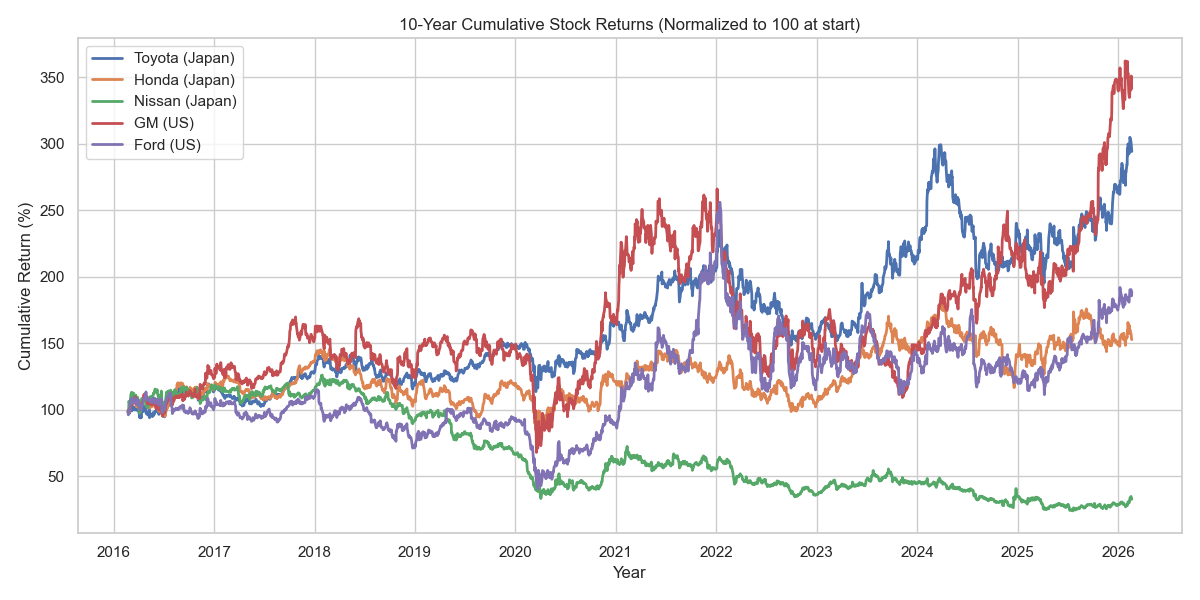
\includegraphics[width=0.9\textwidth]{cumulative_returns.png}
\caption{サンプル開始時点を100に正規化した累積株式収益率。パターンはマクロ局面と企業固有の転換点（特に日産の長期的低迷）を反映する。}
\end{figure}

トヨタは比較的低いボラティリティと強い複利的な上昇軌道を示し、操業規律と現地化がマクロ・ショックを緩和するという見方と整合的である。日産の10年にわたる負のパフォーマンスと極端なドローダウンは、ガバナンス混乱と戦略的不安定性を反映し、為替を含むマクロ金融変数への感応度を増幅しうる。

\section{計量経済学的手法}

為替ショックが株式価値に及ぼす因果効果を推定するため、本稿では二つの補完的アプローチを用いる。(i) Local Projections with Instrumental Variables（LP-IV）により動学的インパルス応答を推定し、(ii) 日銀・FRBの不連続なサプライズを用いたイベントスタディを実施する。

\paragraph{データ}

データセットは10年の期間にわたる日次観測からなる。トヨタ、ホンダ、日産、GM、フォードの株価終値、S\&P~500指数（\^{}GSPC）、USD/JPYスポット（JPY=X）はYahoo Financeから取得する。操作変数は米国2年国債のコンスタント・マチュリティ利回り（DGS2）の日次変化であり、FREDから取得する。株価と為替は日次対数収益率に変換し、2年利回りは差分（ベーシス・ポイント変化）を用いる。

\paragraph{「USD/JPY上昇」ショックの解釈}

以下では「appreciation」ショックはUSD/JPYの正の変化（1ドル当たりの円が増える）を指す。経済的には、\emph{ドル高・円安}である。古典的な輸出モデルでは、USD/JPYの上昇は日本メーカーの価格競争力とドル収益の円換算額を押し上げ、日本の自動車株にプラスに働くはずである。他方、現地化が深い場合、収益と費用が同一通貨圏で一致するため効果は小さくなるはずである。

米国メーカーについては符号は理論的に曖昧である。ドル高は輸入投入財のコストや海外生産費用を低下させうる一方、海外利益の換算額を圧縮し、輸出競争力を弱めうる。本稿の推定結果は、金融政策由来のUSD/JPY変動が株式価値にもたらす\emph{純効果}を示す。

\paragraph{内生性と操作変数の必要性}

USD/JPY変化と株式収益率を単純にOLSで回帰すると、(i) 逆因果（リスク回避局面では株式下落と同時に安全資産として円高が進むなど）と、(ii) 省略変数（リスク選好、コモディティ価格、マクロニュースなど）が両者を同時に動かすことで、推定がバイアスを受ける。

\paragraph{LP-IVの仕様}

本稿は、地平$h \in \{0,1,\ldots,10\}$について、2段階最小二乗（2SLS）によるローカル・プロジェクション推定を行う \citep{jorda2005}。

\paragraph{第1段階（ファーストステージ）.}
内生的なUSD/JPY収益率$X_t$を、米国2年利回りの日次変化$Z_t$で操作し、同時にS\&P~500収益率$W_t$を統制する：
\begin{equation}
X_t = \alpha_0 + \alpha_1 Z_t + \alpha_2 W_t + \nu_t.
\end{equation}
推定値$\widehat{X}_t$は、同時的な株式ショックではなく、金融政策サプライズによって駆動された為替変動を捉えることを意図する。

\paragraph{第2段階（セカンドステージ）.}
各地平$h$について、時点$t-1$から$t+h$までの企業$i$の累積収益率$Y_{t,t+h}$を、$\widehat{X}_t$と$W_t$に回帰する：
\begin{equation}
Y_{t,t+h} = \beta_{0,h} + \beta_{1,h} \widehat{X}_t + \beta_{2,h} W_t + \epsilon_{t+h}.
\end{equation}
系列$\{\beta_{1,h}\}$は、USD/JPYが1\%上昇するショック（ドル高・円安）に対する累積株式反応を与える。

\paragraph{推論.}
累積収益率は地平間で重なり（overlap）を持つため、誤差項は自己相関を含む。そこで、ラグ長を$h+1$に比例させたHAC（Newey--West）標準誤差を用いる。

\paragraph{イベントスタディ設計とショックの選定}

外部検証として、USD/JPYが大きく不連続に動いた8つの日銀・FRBイベント（2013--2024年）について、市場モデルに基づく標準的なイベントスタディ \citep{mackinlay1997} を行う。「通常」収益率は110営業日の推定窓$[-120,-10]$で推定し、異常収益（AR）および累積異常収益（CAR）をイベント窓$[-1,+5]$で算出する。

イベントは、FX市場で顕著な急変を引き起こし、サプライズとして広く解釈されたものを選ぶ。

\paragraph{円安局面（USD/JPYがジャンプして上昇）.}
\begin{enumerate}
\item \textbf{2013年4月4日 -- 日銀「QQEバズーカ」}: 黒田総裁が予想を上回る量的・質的緩和を発表。
\item \textbf{2014年10月31日 -- 日銀追加緩和}: 資産購入のサプライズ拡大により「アベノミクス」緩和を補強。
\item \textbf{2022年8月26日 -- FRBジャクソンホール}: パウエル議長が強いインフレ抑制姿勢を示し、利回り上昇とドル高を誘発。
\item \textbf{2024年3月19日 -- 日銀NIRP/YCCからの退出}: マイナス金利を解除したが、市場は「材料出尽くし」で円安方向に反応。
\end{enumerate}

\paragraph{円高局面（USD/JPYが下落）.}
\begin{enumerate}
\item \textbf{2016年1月29日 -- 日銀NIRP}: マイナス金利導入が逆効果となり、安全資産需要で円高。
\item \textbf{2016年9月21日 -- 日銀YCC}: イールドカーブ・コントロール導入（レジーム転換）で短期的に円高。
\item \textbf{2022年12月20日 -- 日銀YCC修正}: 長期金利変動幅の拡大がサプライズとなり、急速な円高。
\item \textbf{2023年7月28日 -- 日銀YCC柔軟化}: 長期金利上昇を容認し、事実上の引き締めと解釈。
\end{enumerate}

表~\ref{tab:events}はイベント集合を要約する。

\begin{table}[H]
\centering
\caption{ナラティブ・イベントスタディで用いた日銀／FRB政策イベント}
\label{tab:events}
\begin{tabular}{p{2.2cm} p{2.8cm} p{2.4cm} p{6.1cm}}
\toprule
日付 & 機関 & 為替方向 & USD/JPYに関する解釈 \\
\midrule
2013-04-04 & 日銀 & 円安 & 大規模緩和サプライズ；USD/JPY上昇（円安）。 \\
2014-10-31 & 日銀 & 円安 & 追加緩和；USD/JPY上昇。 \\
2016-01-29 & 日銀 & 円高 & NIRPが逆効果；リスクオフで円高。 \\
2016-09-21 & 日銀 & 円高 & YCC導入（レジーム転換）；短期的に円高。 \\
2022-08-26 & FRB & 円安 & タカ派シグナル；利回り上昇；ドル高。 \\
2022-12-20 & 日銀 & 円高 & YCCバンド拡大；急速な円高。 \\
2023-07-28 & 日銀 & 円高 & YCC柔軟化；引き締めと解釈。 \\
2024-03-19 & 日銀 & 円安 & NIRP終了；「材料出尽くし」で円安。 \\
\bottomrule
\end{tabular}
\end{table}

\section{実証結果}

\paragraph{記述的な共動性と還元形の「エクスポージャー・パズル」}

まず単純だが示唆的な事実から始める。日次株式収益率とUSD/JPY変化の無条件相関は、5社すべてでほぼゼロに近い。

\begin{figure}[H]
\centering
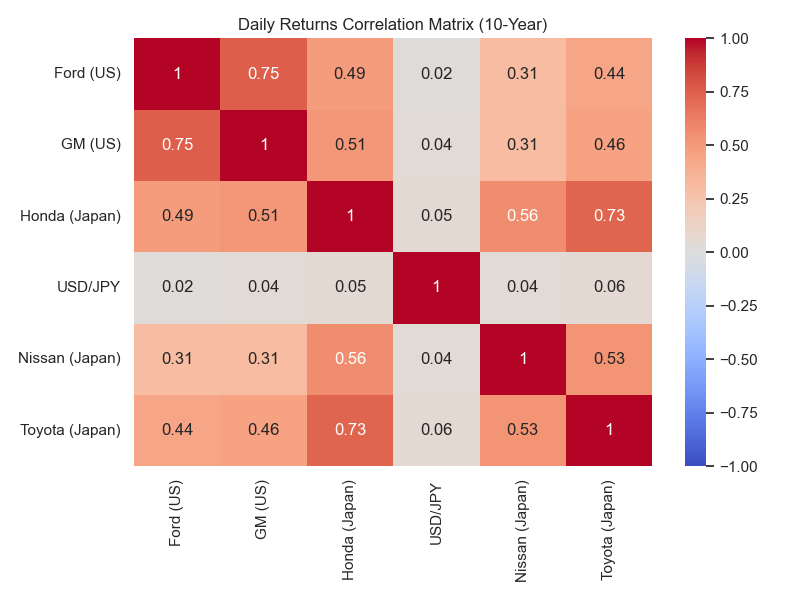
\includegraphics[width=0.75\textwidth]{correlation_matrix.png}
\caption{日次収益率（自動車株とUSD/JPY）のピアソン相関行列。フォード--GMやホンダ--トヨタなど同業内の相関は強い一方、USD/JPYと株式の相関はほぼゼロに近い。}
\end{figure}

二つのパターンが目立つ。第一に、米国2社（フォード--GMの相関$0.75$）と日本企業群（ホンダ--トヨタ$0.73$、日産--トヨタ$0.53$、ホンダ--日産$0.56$）の内部で共動性が強い。第二に、USD/JPYの相関はきわめて小さく、$0.02$から$0.06$の範囲にある。

透明性のため、表~\ref{tab:fxcorr}に各社とUSD/JPYの相関を示す。

\begin{table}[H]
\centering
\caption{日次株式収益率とUSD/JPYの無条件相関}
\label{tab:fxcorr}
\begin{tabular}{lr}
\toprule
企業 & Corr$(r_{i,t},\Delta \log(USD/JPY)_t)$ \\
\midrule
フォード & 0.02 \\
GM & 0.04 \\
ホンダ & 0.05 \\
日産 & 0.04 \\
トヨタ & 0.06 \\
\bottomrule
\end{tabular}
\end{table}

これらの相関を文字通り解釈すれば、為替は自動車株に無関係に見える。しかしそれは誤解を招く。日次の為替変化には多様なショックが混在する。たとえばグローバルなリスク回避に伴う円高は、自動車株の下落と同時に起こりうるが、純粋な通貨換算ショックが与える符号は逆かもしれない。したがって因果識別には、外生的なFX変動の特定の源泉を切り出すことが必要である。

\paragraph{LP-IVインパルス応答：異質で持続的な為替感応度}

図~\ref{fig:lpiv}は、USD/JPYが1\%上昇するショック（ドル高・円安）に対するLP-IVインパルス応答を示す。

\begin{figure}[H]
\centering
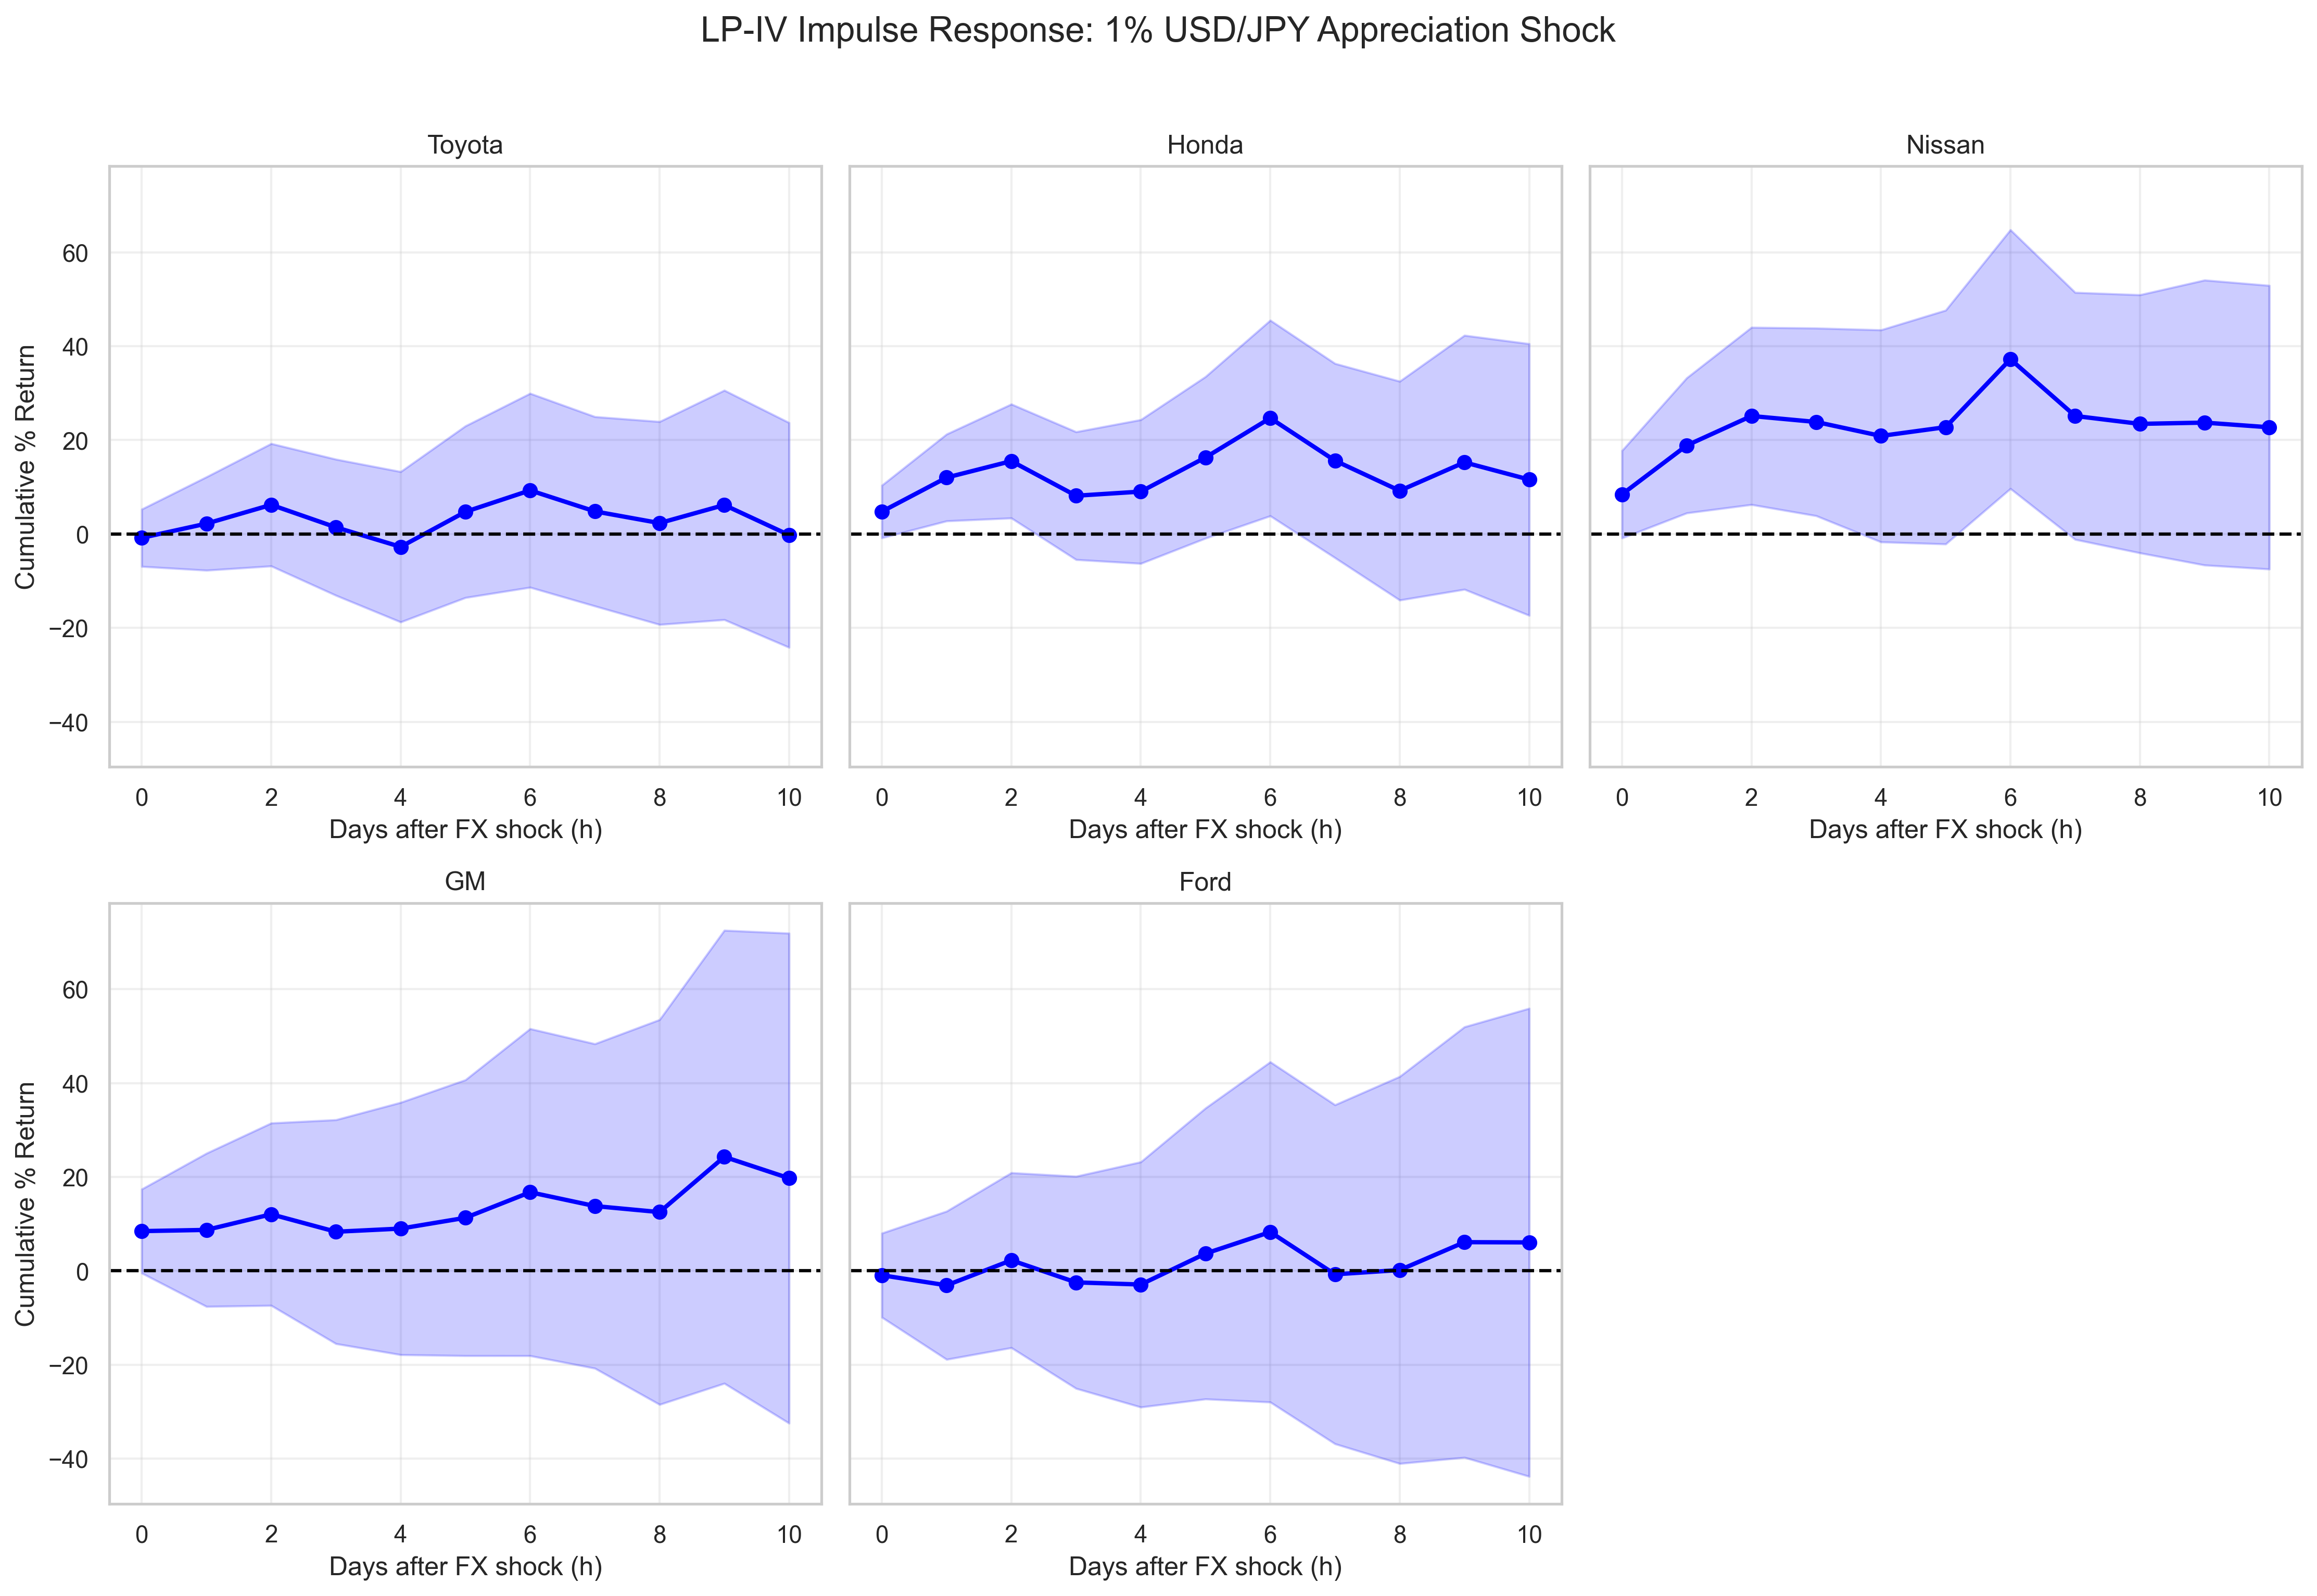
\includegraphics[width=0.9\textwidth]{lp_iv_irf.png}
\caption{USD/JPYが1\%上昇するショック（ドル高・円安）に対するLP-IVインパルス応答。網掛けはHAC頑健な95\%信頼区間を表す。}
\label{fig:lpiv}
\end{figure}

インパルス応答は、還元形相関の結果を覆す。4社は1～2週間の地平で経済的に大きな正の反応を示す一方、トヨタはほぼフラットである。

企業間の順位付けを要約するため、表~\ref{tab:lpivsummary}に$h=10$における最終累積反応を示す。

\begin{table}[H]
\centering
\caption{USD/JPYが1\%上昇するショック（ドル高・円安）に対するLP-IV累積反応（$h=10$）}
\label{tab:lpivsummary}
\begin{tabular}{lr}
\toprule
企業 & 累積反応（\%） \\
\midrule
トヨタ & $-0.24$ \\
フォード & $+6.0$ \\
ホンダ & $+10.7$ \\
GM & $+18.3$ \\
日産 & $+22.6$ \\
\bottomrule
\end{tabular}
\end{table}

\paragraph{トヨタ：オペレーショナル遮断のベンチマーク.}
トヨタの反応は10営業日の地平全体でゼロ近傍を振動し、最終推定値は$-0.24\%$で統計的にゼロと区別できない。これは「深い現地化」と整合的である。北米販売の大部分が北米で生産・調達されていれば、ドル収益はドル費用によって自然にヘッジされる。この場合、ドル円の変動は一部の利益の会計上の換算値を変えるにとどまり、期待される操業キャッシュフローを大きく変えるとは限らない。

\paragraph{ホンダと日産：部分的現地化の下で残るエクスポージャー.}
ホンダと日産は明確な正の反応を示し、最終累積効果はそれぞれ約$+10.7\%$と$+22.6\%$である。点推定は、金融政策由来の円安がこれらの企業にとって利益増加ショックとして解釈されていることを示唆する。両社とも米国内生産を展開してきたが、サプライヤーの深さ、製品ミックス、グローバルな配置が異なる。LP-IVの結果は、連結収益の中に依然として通貨の不一致（unmatched）部分が相対的に大きく、通貨換算と競争価格の効果に晒されているという見方と整合的である。

\paragraph{GMとフォード：理論的符号が曖昧でも正の反応.}
GMとフォードも正の累積反応を示す。ここで重要なのは、対象が単なる会計的「為替エクスポージャー」ではなく、\emph{金融政策によって誘発された}USD/JPY上昇が株式価値に与える因果効果だという点である。正の符号は複数のチャネルで合理化できる。輸入投入財の低下、海外生産の費用がドル建てで低下することによる利幅改善、そして利回り主導のドル高が景気ニュースと相関し、景気循環産業に強く作用する可能性などである。

\paragraph{タイミングと持続性.}
反応は同時点だけで完結せず、数日かけて累積する。日産では第1週で急速に上昇し高止まりし、GMではより緩やかに上昇して後半にピークを迎える。これは期待収益チャネルと整合的である。為替ニュースがまず利幅・換算の期待を変え、その修正が数セッションに分けて株価に織り込まれる。

\paragraph{大きさと不確実性.}
点推定はとりわけ日産とGMで大きい。地平が長くなるほど信頼区間は大きく広がる。これは、重なりを持つ累積収益率の推定ノイズと、操作変数を用いても時間の経過とともに交絡ショックが蓄積するためである。含意は二つある。第一に、単一地平での精密な大きさよりも、企業間の\emph{順位付け}の方が頑健である。トヨタは一貫して最も感応度が低く、日産とGMが最も高い。第二に、推定は特定のタイプのFX変動（短期金利サプライズによって誘発されたもの）の効果であり、あらゆるUSD/JPY変動に普遍的に当てはまる写像ではない。

\paragraph{イベントスタディ：不連続な政策ショックとCARの非対称性}

イベントスタディは、日銀・FRBの不連続なサプライズを用いてナラティブな確認を行う。

\begin{figure}[H]
\centering
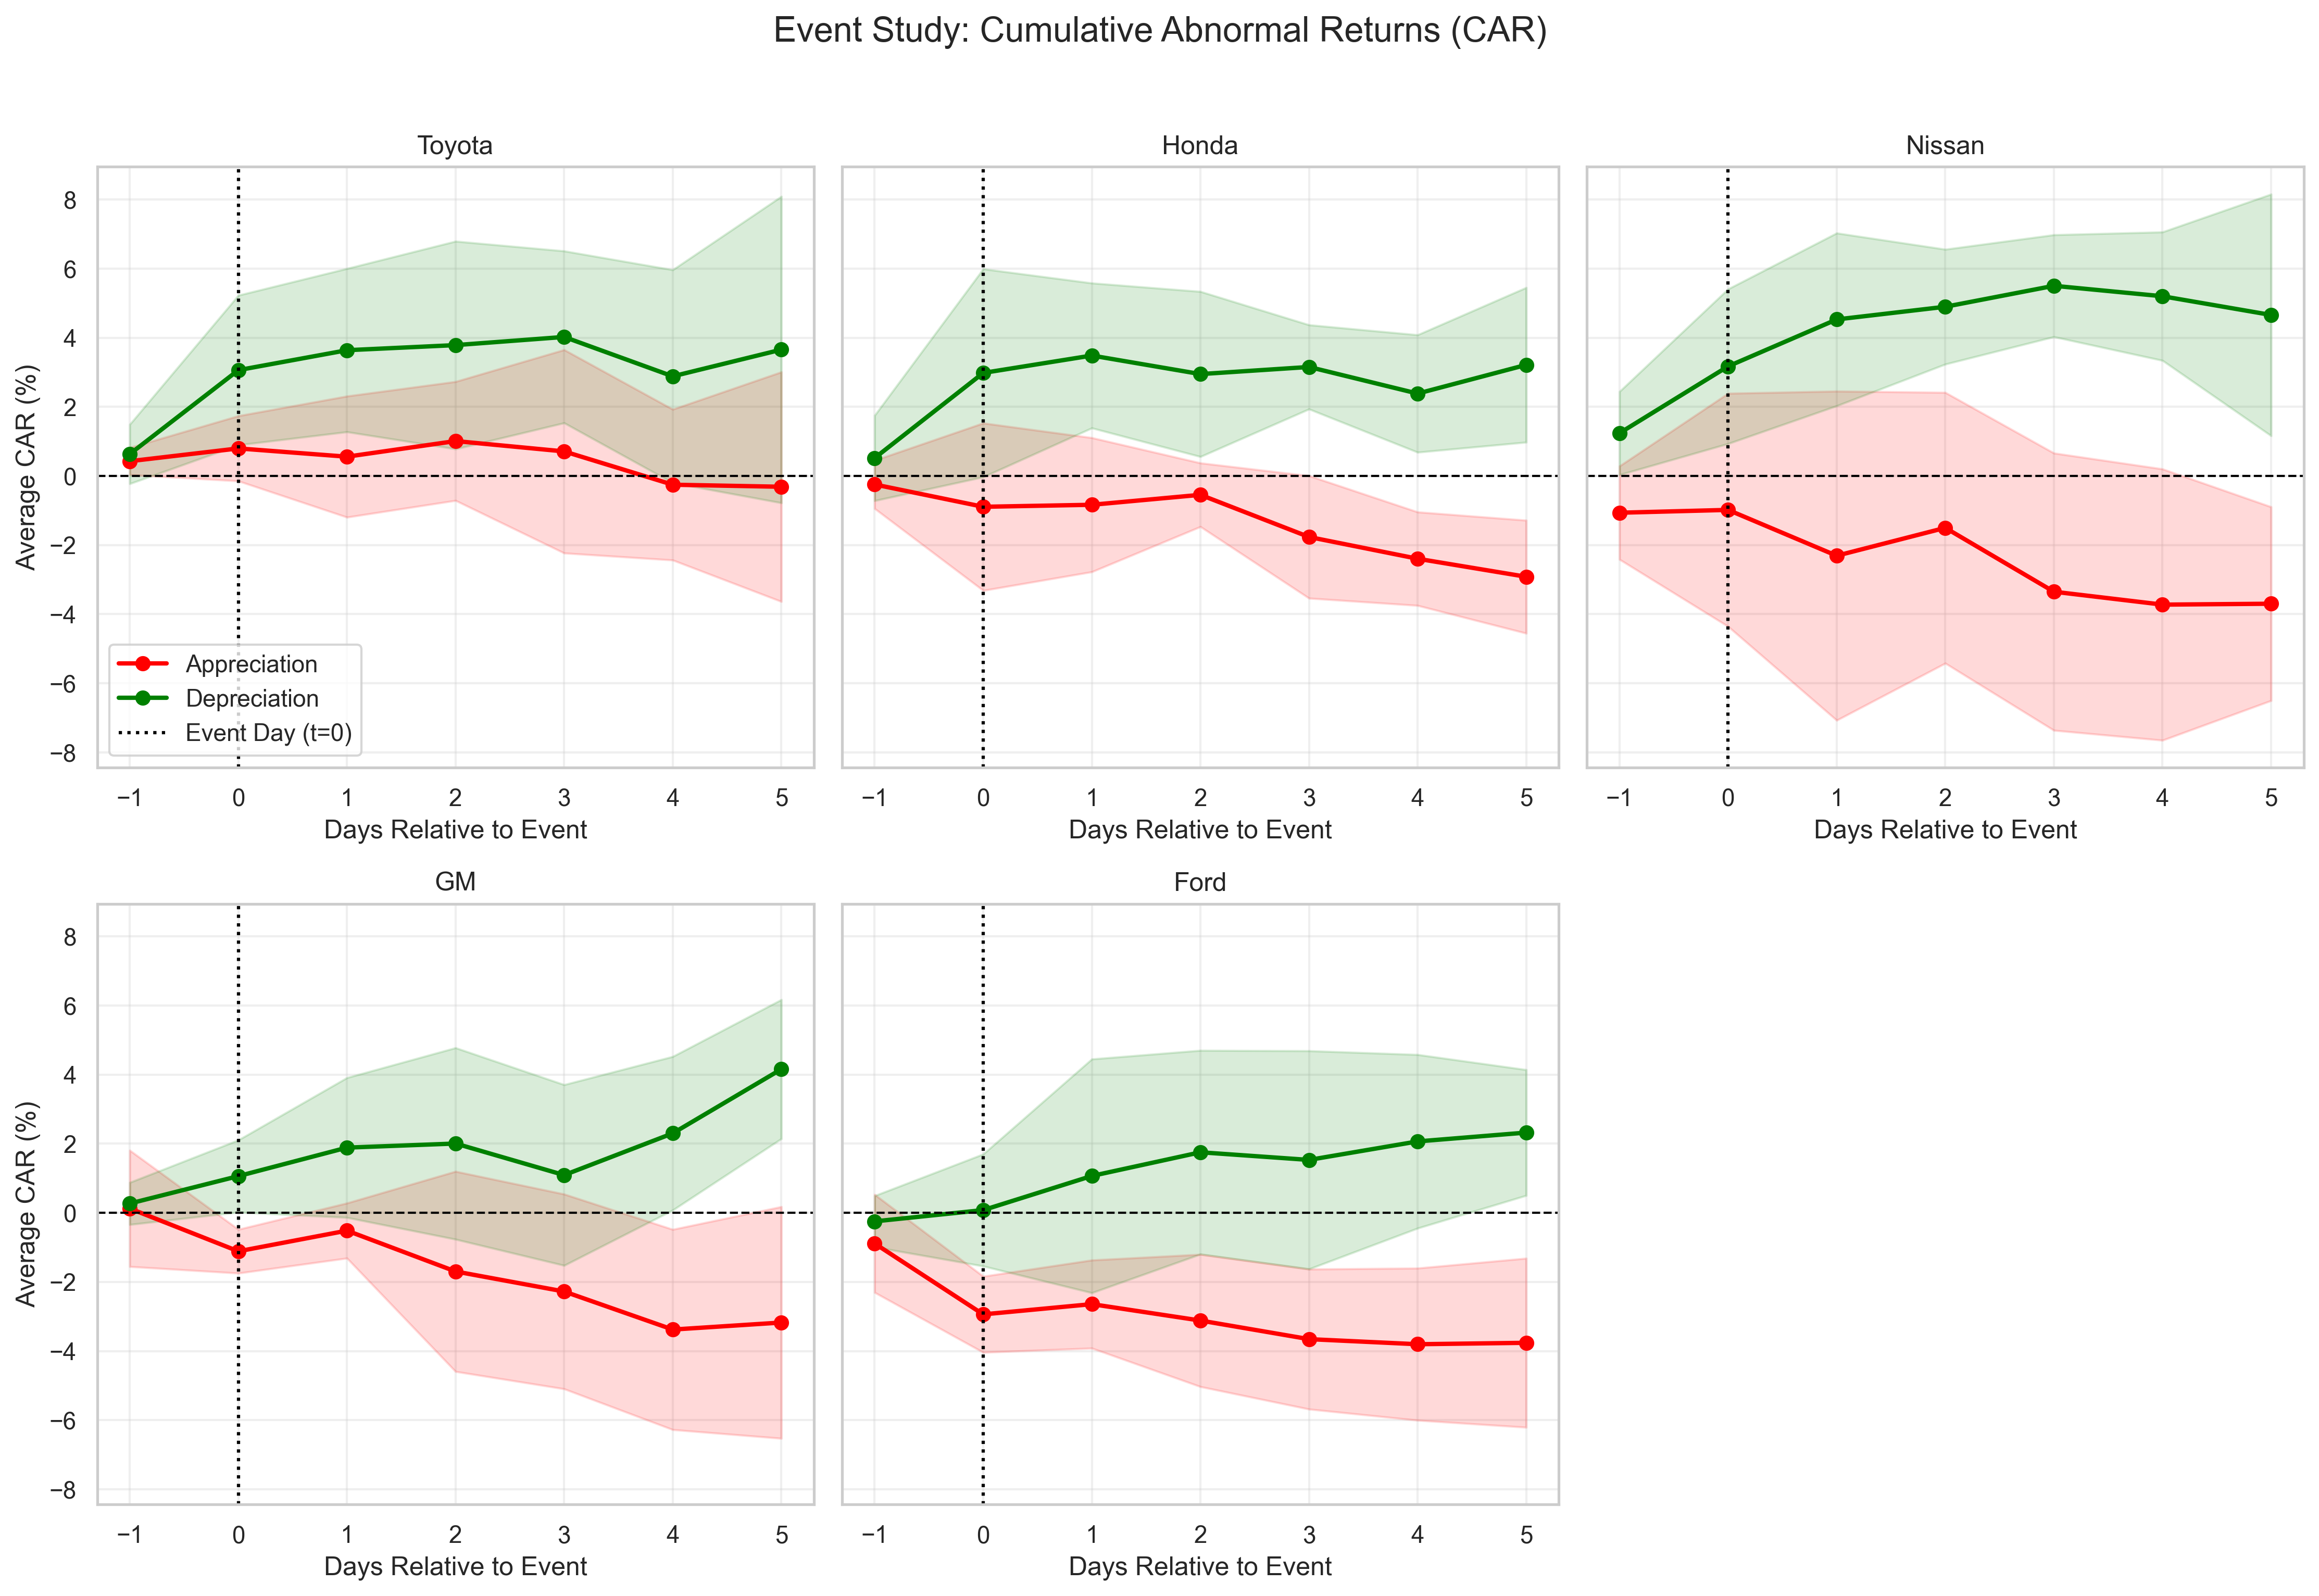
\includegraphics[width=0.9\textwidth]{event_study_car.png}
\caption{日銀／FRBのFXショックイベントの周り（$[-1,+5]$）における平均累積異常収益（CAR）。円安イベント（緑）と円高イベント（赤）に分割。網掛けはイベント間の不確実性バンドを表す。}
\end{figure}

重要な結果は三点である。

\paragraph{(1) トヨタのCARは両レジームでほぼゼロ.}
トヨタの平均CARは、円高イベントの後でおよそ$t=5$時点で$-0.31\%$、円安イベントの後でおよそ$+3.66\%$と小さく、いずれも報告された要約では統計的にゼロと区別できない。これは、操業キャッシュフローが通貨一致している企業に典型的に期待される対称性である。

\paragraph{(2) 「感応的コホート」の強い反応.}
ホンダ、日産、GM、フォードは顕著な非対称性を示す。円高ショックは負のCARを、円安ショックは正のCARを生む。特にホンダと日産は円高イベント後の負の異常パフォーマンスが大きく、円高が利幅圧縮や換算面で不利に働くことと整合的である。

\paragraph{(3) タイミング：反応は複数日にわたって積み上がる.}
CARは$ t=0 $で一気に跳ねるというより、数セッションをかけてドリフトすることが多い。これは情報の段階的な取り込みと整合的である。政策ショックがまずFX市場を動かし、次に投資家が利益見通しを修正し、その結果として異常収益が累積する。

\paragraph{総合：統計結果を貿易史へ接続する}

LP-IVとイベントスタディを併せてみると、メッセージは一貫している。自動車セクターの為替エクスポージャーは存在するが、企業特有性が極めて大きい。トヨタは伝統的な通貨チャネルを実質的に中和している一方、他社は依然として曝されている。

歴史的観点から見れば、これは偶然ではない。「貿易戦争」期は日本メーカーに米国の「国内生産者」になる強いインセンティブを与え、プラザ合意は現地化を数量制約回避の戦術から、通貨ミスアライメントに対する生存戦略的ヘッジへと変質させた。今日のトヨタの際立った遮断は、その長期的戦略コミットメントの帰結として読むのが自然である。

\section{考察：通商ナラティブとリスク管理への含意}

\paragraph{日米自動車政治における「円安優位」論の再検討}

米国の政治議論では、円安が日本の自動車輸出に対する直接的な補助金のように扱われることが多かった。本稿の結果は、より複雑な現実を示唆する。円安は依然として一部企業にとって重要であり、ホンダ、とりわけ日産は意味のある正の感応度を示す。しかしそれは、すべての日本メーカーに一様な優位を与えるものではない。最も大きく象徴的な日本メーカーであるトヨタは、ほとんどエクスポージャーを示さない。すなわち、米国の政治ナラティブの中心に置かれてきた企業ほど、そのナラティブが強調する為替メカニズムの影響を受けにくい。

この点は二つの含意を持つ。第一に、「日本＝輸出モデル」という同質的な前提に基づく通商政策論は、今日ではますます時代遅れである。第二に、現地化によるオペレーショナル・ヘッジの有効性は、長期的なエクスポージャーが過去の貿易摩擦により内生的に形成されうることを意味する。政治的圧力が強く、北米生産に最も投資した企業ほど、通貨感応度を弱めた可能性が高い。

\paragraph{なぜ現地化はエクスポージャーを中和するのか：キャッシュフローの写像}

統計結果を経済構造に接続する最も簡潔な方法は、操業キャッシュフローの通貨構成に注目することである。米国販売によるドル収益を$R^{\$}$、ドル費用を$C^{\$}$とし、ドル建て操業余剰を$\Pi^{\$}=R^{\$}-C^{\$}$とする。日本から輸出する企業では$C^{\$}$が小さく$C^{\yen}$が大きいため、円安は外貨収益の円換算額を押し上げ、価格設定の柔軟性も高めることで$\Pi^{\yen}$を増加させる。現地生産企業では$R^{\$}$と$C^{\$}$がともに大きく、$\Pi^{\$}$はUSD/JPYに対して相対的に鈍感になる。

トヨタのゼロ反応は、北米事業における$R^{\$}$と$C^{\$}$の通貨一致（matched position）が大きいことと整合的である。日産の大きな正の反応は、より大きな不一致成分（日本からの輸出比率が高い、円建てコスト曝露が大きい、あるいはpricing-to-marketで利幅を安定化させにくい等）を示唆する。

\paragraph{限界と頑健性に関する留意点}

大きさを解釈する際には二つの注意点がある。

第一に、IVが識別するのは\emph{利回り主導}の為替変動の効果である。2年利回りのショックが割引率や需要チャネルを通じて自動車株に直接影響する場合、排除制約（exclusion restriction）は完全ではない可能性がある。S\&P~500で広いリスクオン／オフを統制しているが、産業固有の金利感応度は残りうる。

第二に、多国籍企業の測定には留意が必要である。日本株を米国上場のADRで測定している場合、基礎となる円建て株価が不変でも、USD/JPYがドル建て収益率に機械的影響を与えうる。ただし、本稿でホンダと日産が正に反応している（機械的にはむしろ負になり得る）ことは、これらのイベントではファンダメンタルズ効果が優勢である可能性を示す。将来の研究では、本国市場の円建て株価で分析を再現し、株式収益率を「現地株価変動」と「通貨成分」に明示的に分解することが有益である。

自然な拡張として、非線形性とレジーム依存性を検討できる。危機局面（円が安全通貨として振る舞う）と拡張局面（金利差が支配的）では、エクスポージャーが異なる可能性がある。

\section{結論}

日米自動車関係は、貿易摩擦と通貨政治の長い相互作用によって形作られてきた。オイルショック後の輸入浸透、自主規制、プラザ合意、そして数十年にわたるトランスプラント拡大に至るまで、政策ショックは繰り返し生産の地理を変えてきた。本稿は、それらの歴史的調整が現代の金融市場における感応度として可視化されることを示す。

LP-IVとイベントスタディにより、為替エクスポージャーの強い企業間異質性を確認した。ホンダ、日産、GM、フォードは、金融政策由来のUSD/JPY上昇（円安）に対して株価が正に反応する一方、トヨタは実質的に遮断されている。これは「為替エクスポージャー・パズル」に企業レベルの解を与える。すなわち、エクスポージャーは「日本メーカー」や「輸出企業」に固有の一様な特徴ではなく、現地化を含む操業構造と戦略の内生的帰結である。

政策当局にとっての含意は、通商紛争における為替論はターゲットを絞り、証拠に基づくべきだということである。通貨チャネルは一部企業にとって現実であるが、他社にはほとんど無関係である。企業と投資家にとっては、「マクロ」リスクはデリバティブ市場でヘッジされるだけでなく、数十年単位の生産・サプライヤー戦略によって設計し、場合によっては消し去ることができる、という点が示唆される。

\bibliographystyle{apalike}

\bibliography{references}

\end{document}
